\documentclass[11pt]{article}

\usepackage{amsmath}
\usepackage{amssymb}
\usepackage{color}
\usepackage{listings}
\usepackage{graphicx}


\textwidth=6.5in
\textheight=9in
\topmargin=-0.8in
\headheight=15.75pt
\headsep=.35in
\oddsidemargin=0.0in
\evensidemargin=0.0in

\newcommand{\Complex}{\mathbb{C}}
\newcommand{\Real}{\mathbb{R}}
\newcommand{\Dpt}{D_{+t}}
\newcommand{\Dmt}{D_{-t}}
\newcommand{\Dzt}{D_{0t}}
\newcommand{\Dpx}{D_{+x}}
\newcommand{\Dmx}{D_{-x}}
\newcommand{\Dzx}{D_{0x}}
\newcommand{\Oc}{\mathcal{O}}
\newcommand{\dx}{\Delta x}
\newcommand{\dt}{\Delta t}
\newcommand{\vnpj}{v^{n+1}_j}
\newcommand{\vnjp}{v^n_{j+1}}
\newcommand{\vnjm}{v^n_{j-1}}
\newcommand{\vnj}{v^n_j}
\newcommand{\vnjpp}{v^n_{j+2}}
\newcommand{\vnjmm}{v^n_{j-2}}
\newcommand{\ux}{u_x(0)}
\newcommand{\uxx}{u_{xx}(0)}
\newcommand{\uxxx}{u_{xxxx}(0)}
\newcommand{\ufour}{u^{(4)}(0)}
\newcommand{\ufive}{u^{(5)}(0)}


\begin{document}
\begin{flushright}
\small{MATH-6840\\
Vignesh Ramakrishnan\\
RIN: 662028006\\
{\bf Due: Monday February 7, 2022}}
\end{flushright}

\begin{center}
\large{Problem Set 3}\\
\end{center}

NPDE is the textbook {\em Numerical Partial Differential Equations}. Submissions are due in the LMS, and must be typeset (e.g. \LaTeX).

\begin{enumerate}
  %%%%%
  %%%%%
  %%%%%
  \item (10 pts.) {\color{red}Consider the smooth function} $u(x)$ {\color{red}to be known at integer grid points} $x_j=j\dx$ {\color{red}and use the notation} $u_j=u(x_j)$
  \begin{enumerate}
    \item {\color{blue}Is it possible to approximate} $u_{x}(0)$ {\color{blue}with error} $\Oc(\dx^3)${ \color{blue}for general} $u(x)$ {\color{blue}using solution values} $u_j$, {\color{blue}for} $j=-1,0,1${\color{blue}?}\\
    
    This exercise is to figure out if $\ux$ can be approximated with error $\Oc(\dx^3)$ using solution values $u_j$ for $j = -1,0,1$.
    \begin{align*}
    \text{Let,  } \ux = & \ au(-\dx) + bu(0) + cu(\dx) + \text{Error} \\
    \ux = & \ a\left[u(0) -\dx\ux + \frac{\dx^2}{2!}\uxx - \frac{\dx^3}{3!}\uxxx + ....\right]\\
    & + bu(0) \\
    & + c\left[u(0) + \dx\ux + \frac{\dx^2}{2!}\uxx + \frac{\dx^3}{3!}\uxxx\right] + \text{Error} \\
    \ux = & \ \left(a + b + c\right)u(0)  + \dx\left(-a+c\right)\ux \\
    & + \frac{\dx^2}{2!}\left(a+c\right)\uxx + \frac{\dx^3}{3!}\left(-a+c\right)\uxxx + ... \ ... + \text{Error}
    \end{align*}
    Matching the coefficients on the LHS with the coefficients on RHS results in 
   \begin{align*}
  & a + b + c = 0 \\
   & \dx \left(-a + c\right) = 1 \\
   & \frac{\dx^2}{2!}\left(a+c\right) = 0 \\
   & \text{Solving for, } a, b, \text{and, } c \text{ gives} \\
   & a = \frac{-1}{2\dx} \\
   & b = 0 \\
   & c = \frac{1}{2\dx} 
   \end{align*}
    Substituting this back in the previous equation, we can find what Error term is, 
    \begin{align*}
    \ux = & \ 0 + \ux + 0 + \frac{\dx^3}{3!}\frac{2}{2\dx}\uxxx + \frac{\dx^5}{5!}\frac{2}{2\dx} \ufive + ... \ ... + \text{Error} \\
    \text{Error} = & \ -\dx^2\left[\frac{1}{2!}\uxxx + \frac{\dx^2}{5!}\ufive + ... \ + ...\right] = \Oc(\dx^2)
    \end{align*}
    Even if all the three points are used, it is impossible to get an accuracy beyond $\Oc(\dx^2)$.
    
    \item {\color{blue}Under what restrictions on} $u(x)$ {\color{blue}can one approximate} $u_{x}(0)$ {\color{blue}with error} $\Oc(\dx^3)$ {\color{blue}using solution values} $u_j$, {\color{blue}for} $j=-1,0,1${\color{blue}?} \\
    
    If the smooth function $u(x)$ is a polynomial of order 2, like $u(x) = a_0 + a_1x + a_2x^2$, then $\uxx = 2a_2$ and $\uxxx = 0$. In this case, the finite difference approximation developed should be of $\Oc(\dx^3)$ accuracy. \\
    
    \item {\color{blue}Using the solution values }$u_j$, {\color{blue}for} $j=-2,-1,0,1,2$, {\color{blue}derive as accurate an approximation to }$u_{x}(0)$ {\color{blue}as possible. What is the order of accuracy?} \\
    
    In order to get an approximation as accurate as possible, all points $j = -2,-1,0,1,2$ should be used.
    \begin{align*}
    \ux = & \ au(-2\dx) + bu(-\dx) + cu(0) + du(\dx) + eu(2\dx) + \text{Error} \\
    = &  \ a\left[u(0) -2\dx\ux + \frac{(2\dx)^2}{2!}\uxx - \frac{(2\dx)^3}{3!}\uxxx + .... \right] \\
    & + b\left[u(0) -\dx\ux + \frac{\dx^2}{2!}\uxx -\frac{\dx^3}{3!}\uxxx + .... \right] \\
    & + cu(0) \\
    & + d\left[u(0) + \dx\ux + \frac{\dx^2}{2!}\uxx + \frac{\dx^3}{3!}\uxxx + ...\right] \\
    & + e\left[u(0) + 2\dx\ux + \frac{(2\dx)^2}{2!}\uxx + \frac{(2\dx)^3}{3!}\uxxx + ... \right] + \text{Error} \\
    \ux = & \ \left(a+b+c+d+e\right)u(0) + \dx\left(-2a-b+d+2e\right)\ux + \\
    & \frac{\dx^2}{2!}\left(4a+b+d+4e\right)\uxx + \frac{\dx^3}{3!}\left(-8a-b+d+8e\right)\uxxx + \\
    & \frac{\dx^4}{4!}\left(16a+b+d+16e\right)\ufour + ... \ ... + \text{Error}
    \end{align*}
   Equating coefficients on LHS and RHS results in solving the set of linear equations, 
   \begin{align*}
   & a+b+c+d+e = 0 \\
   & \dx \left(-2a-b+d+2e\right) = 1\\
   & 4a+b+d+4e = 0 \\
   & -8a-b+d+8e = 0 \\
   & 16a +b+d+16e = 0 
   \end{align*} 
   Solving for the variables yields, 
   \begin{align*}
    &  a = \frac{1}{12\dx} , b = \frac{-2}{3\dx} , c = 0 , d = \frac{2}{3\dx} , e = \frac{-1}{12\dx} \\ \\
   & \ux = \frac{u(-2\dx)-8u(-\dx)+ 8u(\dx) - u(2\dx)}{12\dx} + \text{Error} 
   \end{align*}
   Expanding these terms further gives,
   \begin{align*}
   \ux = & \ux + a\left[\frac{(2\dx)^4}{4!} \ufour - \frac{(2\dx)^5}{5!}\ufive + ... \right] \\
   & + b\left[\frac{\dx^4}{4!}\ufour - \frac{\dx^5}{5!}\ufive + ...\right] \\
   & + d\left[\frac{\dx^4}{4!}\ufour + \frac{\dx^5}{5!}\ufive + ...\right] \\
   & + e\left[\frac{(2\dx)^4}{4!}\ufour + \frac{(2\dx^5)}{5!}\ufive + ...\right] + \text{Error} \\
   0 = & \left(a+e\right)\left[\frac{(2\dx)^4}{4!}\ufour + \frac{(2\dx)^6}{6!}u^{(6)}(0) + ...\right] \\
   & \left(b+d\right)\left[\frac{\dx^4}{4!}\ufour + \frac{\dx^6}{6!}u^{(6)}(0) + ... \right] \\
   & \left(-a+e\right)\left[\frac{(2\dx)^5}{5!}\ufive + \frac{(2\dx)^7}{7!}u^{(7)}(0) + ...\right] \\
   & \left(-b+d\right)\left[\frac{\dx^5}{5!}\ufive + \frac{\dx^7}{7!}u^{(7)}(0) + ...\right] + \text{Error}\\
   & \text{Here, } a+e = b+d = 0 \text{ and substituting the variables give,}\\
   \text{Error} = & \frac{\dx^4}{6}\left[\frac{2^5}{5!}\ufive + \frac{2^7\dx^2}{7!}u^{(7)}(0) + ...\right] \\
   & - \frac{4\dx^4}{3}\left[\frac{1}{5!}\ufive + \frac{\dx^2}{7!}u^{(7)}(0) + ...\right] = \Oc(\dx^4)
   \end{align*}
   
    \item {\color{blue}Using the solution values }$u_j$, {\color{blue}for} $j=-2,-1,0,1,2$, {\color{blue}derive as accurate an approximation to }$u_{xxx}(0)$ {\color{blue}as possible. What is the order of accuracy?} \\
    
    Following the same procedure as above and matching coefficients will lead to the system of linear equations,
    \begin{align*}
    & a+b+c+d+e = 0 \\
    & -2a-b+d+2e = 0 \\
    & 4a+b+d+4e = 0 \\
    & -8a-b+d+8e = 0 \\
    & 16a+b+d+16e = 0 
    \end{align*}
    Solving,
    \begin{align*}
    a = \frac{-1}{2\dx^3}, b = \frac{1}{\dx^3}, c = 0, d = \frac{-1}{\dx^3}, e = \frac{1}{2\dx^3} \\ \\
    \uxxx = \frac{-u(-2\dx) + 2u(-\dx) -2u(\dx) + u(2\dx)}{2\dx^3}
    \end{align*}
    Substituting these terms and expanding once again yields,
    \begin{align*}
    \uxxx = & \ \uxxx + a\left[ -\frac{(2\dx)^5}{5!}\ufive + \frac{(2\dx)^6}{6!}u^{(6)}(0) + ... \ ...\right] \\
     & b\left[-\frac{\dx^5}{5!}\ufive + \frac{\dx^6}{6!}u^{(6)}(0) + ... \ ...\right] \\
     & d\left[\frac{\dx^5}{5!} \ufive + \frac{\dx^6}{6!}u^{(6)}(0)+ ... \ ...\right] \\
     & e\left[\frac{(2\dx)^5}{5!}\ufive + \frac{(2\dx)^6}{6!}u^{(6)}(0) +... \ ... \right] + \text{Error} \\
     0 = &\ \frac{1}{\dx^3}\left[\frac{(2\dx)^5}{5!}\ufive + \frac{(2\dx)^7}{7!}u^{(7)}(0) + ... \ ...\right] \\
     & - \frac{2}{\dx^3}\left[\frac{\dx^5}{5!}\ufive + \frac{\dx^7}{7!}u^{(7)}(0) + ... \ ... \right] + \text{Error} \\
     \text{Error} = & \Oc(\dx^2)
    \end{align*}
    
  \end{enumerate}
  
  %%%%%
  %%%%%
  %%%%%
  \item(15 pts.) {\color{red}Again consider the smooth function }$u(x)$ {\color{red}to be known at integer grid points }$x_j=j\dx$ {\color{red}and continue to use the notation} $u_j=u(x_j)$.
  \begin{enumerate}
    \item {\color{blue}Derive an infinite expansion for the exact value of} $u_{xx}(0)${ \color{blue}using the discrete operators }$D_{\pm}$ {\color{blue}and} $D_0$ {\color{blue}and assuming} $u_j$ {\color{blue}is know at all relevant locations. }\\
    \begin{align*}
    \Dpx\Dmx u(x_j) = & \frac{u_{j+1}-2u_j + u_{j-1}}{\dx^2} \\
    = & \ \frac{1}{\dx^2}\left[2 \frac{\dx^2}{2!}u_{xx}(x_j) + 2\frac{\dx^4}{4!}u_{xxxx}(x_j) + ... ...\right] \\
    = & \ u_{xx}(x_j) + \frac{2\dx^2}{4!}u_{xxxx}(x_j) + \frac{2\dx^4}{6!}u^{6}(x_j) + .... \\
    u_{xx}(x_j) = & \ \Dpx\Dmx u_j - \frac{2\dx^2}{4!} u_{xxxx}(x_j) - \frac{2\dx^4}{6!} u^{(6)}(x_j) + .... \\
    u_{xx}(x_j) = & \ \Dpx\Dmx u_j - \frac{2\dx^2}{4!} \left(\Dpx\Dmx\right)^2u_j - \frac{2\dx^4}{6!}\left(\Dpx\Dmx\right)^3u_j - .... ... \\
    u_{xx}(x_j) = & \ \left[ \sum_{m=0}^{\infty} \alpha_m \dx^{2m} \left(\Dpx\Dmx\right)^{m+1}\right]u_j
    \end{align*}
    \item {\color{blue}Using the representation in (a) above, derive a nonlinear equation whose solution gives the coefficients in the expansion in (a). }\\
    \begin{align*}
    u = & \ \hat{u}e^{ikx} \\
    u_x =  & \ ik u \\
    u_{xx} = & \ -k^2u \\
    \Dpx\Dmx u_j = & \frac{-4}{\dx^2}\sin^2\left(\frac{\xi}{2}\right) u_j \\
    -k^2u_j = & \sum_{m=0}^{\infty} \alpha_m \dx^{2m} \frac{1}{\dx^2 \dx^2} \left(-4\sin^2\left(\frac{\xi}{2}\right)\right)^{m+1} u_j \\
    -\xi^2 = & \sum_{m=0}^{\infty} \alpha_m\left(-4\sin^2\left(\frac{\xi}{2}\right)\right)^{m+1}
    \end{align*}
    $$ \xi^2 + \sum_{m=0}^{\infty} \alpha_m\left(-4\sin^2\left(\frac{\xi}{2}\right)\right)^{m+1} = 0$$
    \item {\color{blue}Using Taylor series, solve for the coefficients in your expansion and derive a 10th order accurate approximation to }$u_{xx}(0)$.{ \color{blue}Present the discrete approximation. Note you are permitted to use symbolic software such as Maple or Mathematica.} \\
    
    I don't have Mathematica or Maple installed in my laptop, so I used online services (emathhelp.net) to compute the Taylor series expansions in order to derive a 10th order accurate approximation to $\uxx$. \\
    Let, $\xi = 2\eta$:
    \begin{align*}
    0 = & \ \xi^2 + \sum_{m=0}^{\infty} \alpha_m\left(-4\sin^2\left(\frac{\xi}{2}\right)\right)^{m+1} \\
    = & \ 4\eta^2 + \sum_{m=0}^{\infty} \alpha_m\left(-4\sin^2\eta\right)^{m+1}  \\
    \end{align*}
   \begin{align*}
   0 = 4\eta^2 -4\alpha_0 \eta^2 & + \frac{4\alpha_0}{3}\eta^4 - \frac{8\alpha_0}{45}\eta^6 + \frac{4\alpha_0}{215}\eta^8  - \frac{8\alpha_0}{14175}\eta^{10} + ...\ .... \\
   & + 16\alpha_1 \eta^4 - \frac{32\alpha_1}{3}\eta^6 + \frac{16\alpha_1}{5}\eta^8 - \frac{544\alpha_1}{945}\eta^{10} + ... \ .... \\  
   & - 64\alpha_2 \eta^6 + 64\alpha_2 \eta^8 - \frac{448\alpha_2}{15}\eta^{10} + ...\ .... \\
   & + 256\alpha_3 \eta^8 - \frac{1024\alpha_3}{3}\eta^{10} + ... \ .... \\
   & - 1024\alpha_4 \eta^{10} + ... 
   \end{align*}	
Gathering all coefficients and setting  them to 0 results in: 
\begin{align*}
0 = (4-4\alpha_0) \eta^2 & + \left(\frac{4\alpha_0}{3} + 16\alpha_1\right)\eta^4 -\left(\frac{8\alpha_0}{45} + \frac{32\alpha_1}{3} + 64\alpha_2 \right)\eta^6 \\
& + \left(\frac{4\alpha_0}{215} + \frac{16\alpha_1}{5} + 64\alpha_2 + 256\alpha_3\right)\eta^8 + \\
& - \left(\frac{8\alpha_0}{14175} + \frac{448\alpha_2}{15} + \frac{448\alpha_2}{15} + \frac{1024\alpha_3}{3} + 1024\alpha_4 \eta^{10} \right)\eta^{10} + ... \ ....
\end{align*}

Solving for the coefficients,
\begin{align*}
\alpha_0 &= 1 \\
\alpha_1 &= -0.0833 \\
\alpha_2 &= 0.0111 \\
\alpha_3 &= -0.0018 \\
\alpha_4 &= 3.1746\times 10^{-4} \\ 
\text{Therefore} &, \\
\uxx & = \alpha_0\Dpx\Dmx u_j + \alpha_1 \dx^2 \left(\Dpx\Dmx\right)^2 u_j + \\
& \ \alpha_2 \dx^4  \left(\Dpx\Dmx\right)^3 u_j  + \alpha_3 \dx^6 \left(\Dpx\Dmx\right)^4 u_j + \\
& \  \alpha_4 \dx^8 \left(\Dpx\Dmx\right)^5 u_j + \Oc(\dx^{10}) 
\end{align*}

  \end{enumerate}
  
  %%%%%
  %%%%%
  %%%%%
  \item(10 pts.) {\color{red}\em Adopted from NPDE exercise 1.5.12:}
  \begin{enumerate}
    \item {\color{blue}Write a code to approximately solve }
      \begin{align*}
        u_t & = \nu u_{xx}, \qquad\qquad x\in(0,1), \hspace{0.5in} t>0\\
        u(x,0) & = \sin(2\pi x), \hspace{.35in} x\in(0,1)\\
        u(0,t) & = 0, \hspace{2in} t\ge 0 \\
        u(1,t) & = 0, \hspace{2in} t\ge 0.
      \end{align*}
      {\color{blue}Use the grid} $x_j=j\Delta x$, {\color{blue}with} $j=-1,0,1,\ldots,N,N+1${\color{blue}, and }$\Delta x = 1/N$ {\color{blue}(as described in the text), and apply the fourth-order centered spatial discretization with forward Euler time integration for }$j=1,2,\ldots,N-1${\color{blue}, (BCs specified below) i.e.}
      \begin{align*}
        \Dpt v_j^n = \nu\Dpx\Dmx\left(I-\frac{\dx^2}{12}\Dpx\Dmx\right) v_j^n.
      \end{align*}
     The scheme given above can be decomposed into the following format
     \begin{align*}
     \Dpt\vnj = & \ \nu \Dpx\Dmx\left(I\vnj - \frac{\dx^2}{12}\frac{\vnjp -2\vnj + \vnjm}{\dx^2}\right) \\
     = & \ \nu \left[\frac{\vnjp -2\vnj + \vnjm}{\dx^2} -\frac{1}{12}\left(\Dpx\Dmx\vnjp -2\Dpx\Dmx \vnj + \Dpx\Dmx \vnjm\right)\right] \\
     = & \ \nu\left[\frac{\vnjp -2\vnj + \vnjm}{\dx^2}  -\frac{1}{12} \left\{\frac{\vnjpp -4\vnjp + 6\vnj -4\vnjm + \vnjmm}{\dx^2} \right\} \right] \\
     \vnpj = & \ \vnj + \frac{\nu \dt}{12 \dx^2}\left(-\vnjpp + 16\vnjp -30\vnj + 16\vnjm - \vnjmm \right)
     \end{align*}
      A fourth order scheme for all the internal nodes $(j=1,2,3,...,N-1)$and a second order scheme for boundary nodes is applied and the MATLAB code of the same is attached below. For the boundary nodes a second order accurate central difference $u_{xx}$ approximation is used. It is derived at the left and the right boundary as follows,
      \begin{align*}
      u_{xx}(0) = & \ \frac{v^n_{1}-2v^n_0+v^n_{-1}}{\dx^2} + \Oc(\dx^2)\\
      u_{xx}(N) = &\ \frac{v^n_{N+1} - 2v^n_N + v^n_{N-1}}{\dx^2} + \Oc(\dx^2)\\  
      \end{align*}
      As described above, ghost nodes ($v^n_{-1}, v^n_{N+1}$) are introduced and they are calculated using the compatibility boundary condition technique and that is described in part.b) of this question.  
      
    \lstinputlisting[language=Matlab, numbers=left, stepnumber=1, firstline=1,caption={Heat Equation - Order 4 (Q.3b)},label=code:myCode,frame=single]{HeatEqn_Order4.m}   
      
    \item {\color{blue}Set} $\nu=1/6$, $\dt=0.02$, {\color{blue}and} $N=10$. {\color{blue}Define ghost values using }
      \begin{align*}
        v_{-1}^n & = 2v_0^n-v_1^n\\
        v_{0}^n & = 0\\
        v_{N}^n & = 0\\
        v_{N+1}^n & = 2v_{N}^n-v_{N-1}^n,
      \end{align*}
      {\color{blue}and compute approximate solutions at }$t=0.06$, $t=0.1$, {\color{blue}and }$t=0.9$.\\
      
     The approximate solutions generated using this scheme are presented in Fig~\ref{fig:q3b}
      \begin{figure}[htp]
      \begin{center}
      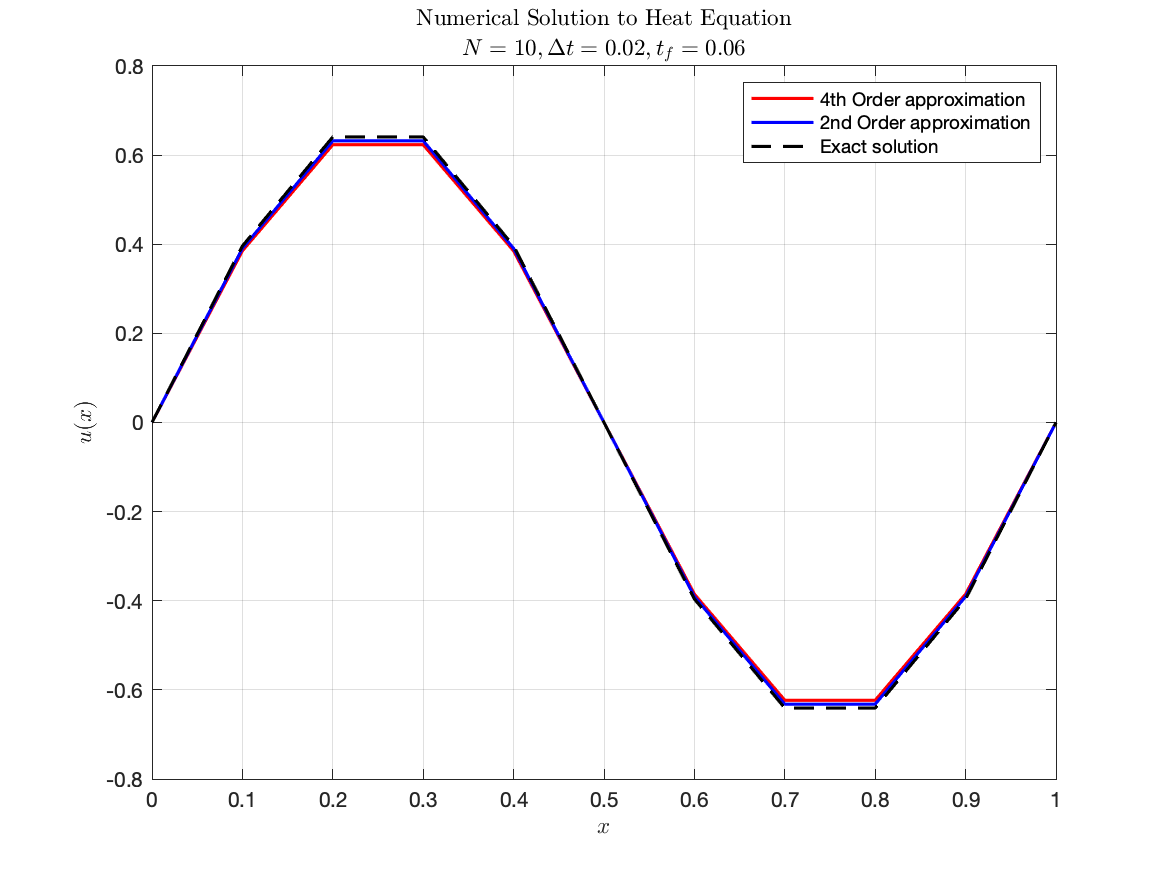
\includegraphics[width=3.8in]{q3_1} \\
      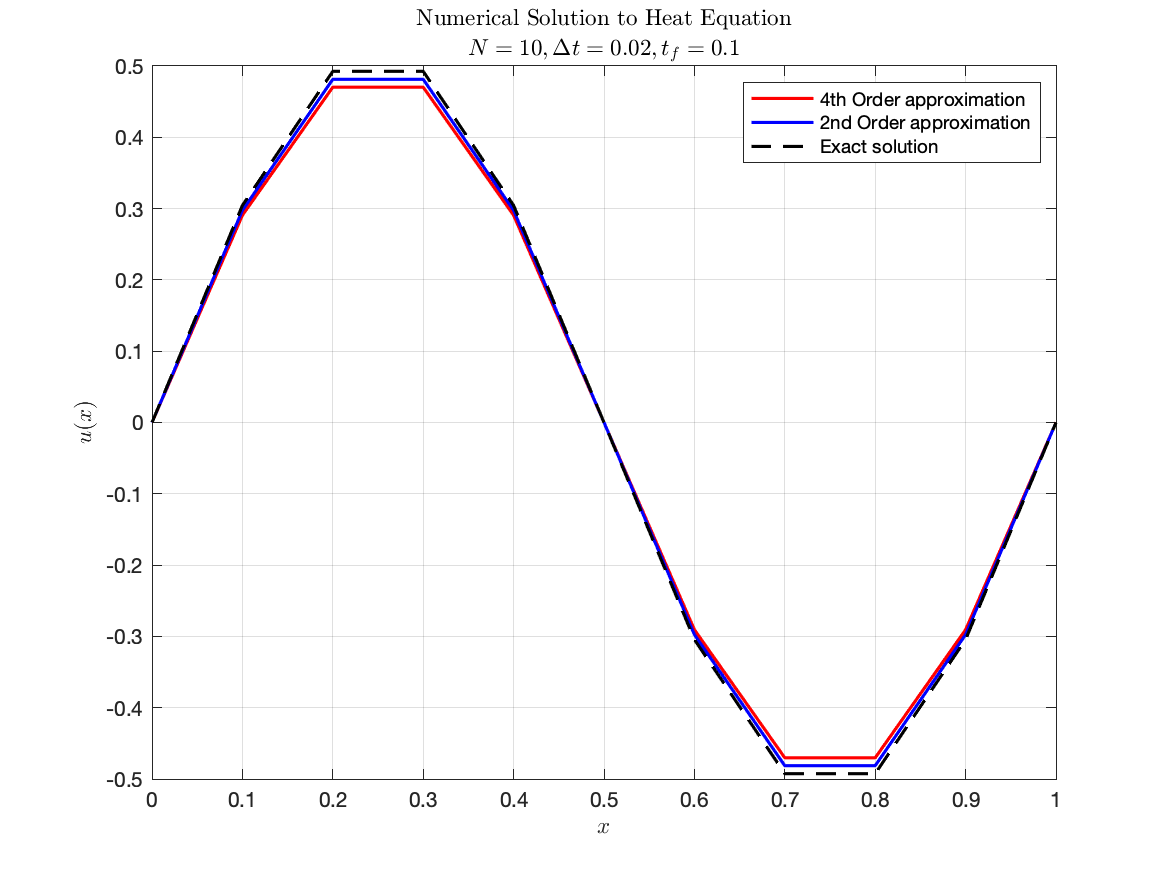
\includegraphics[width=3.8in]{q3_2} \\
      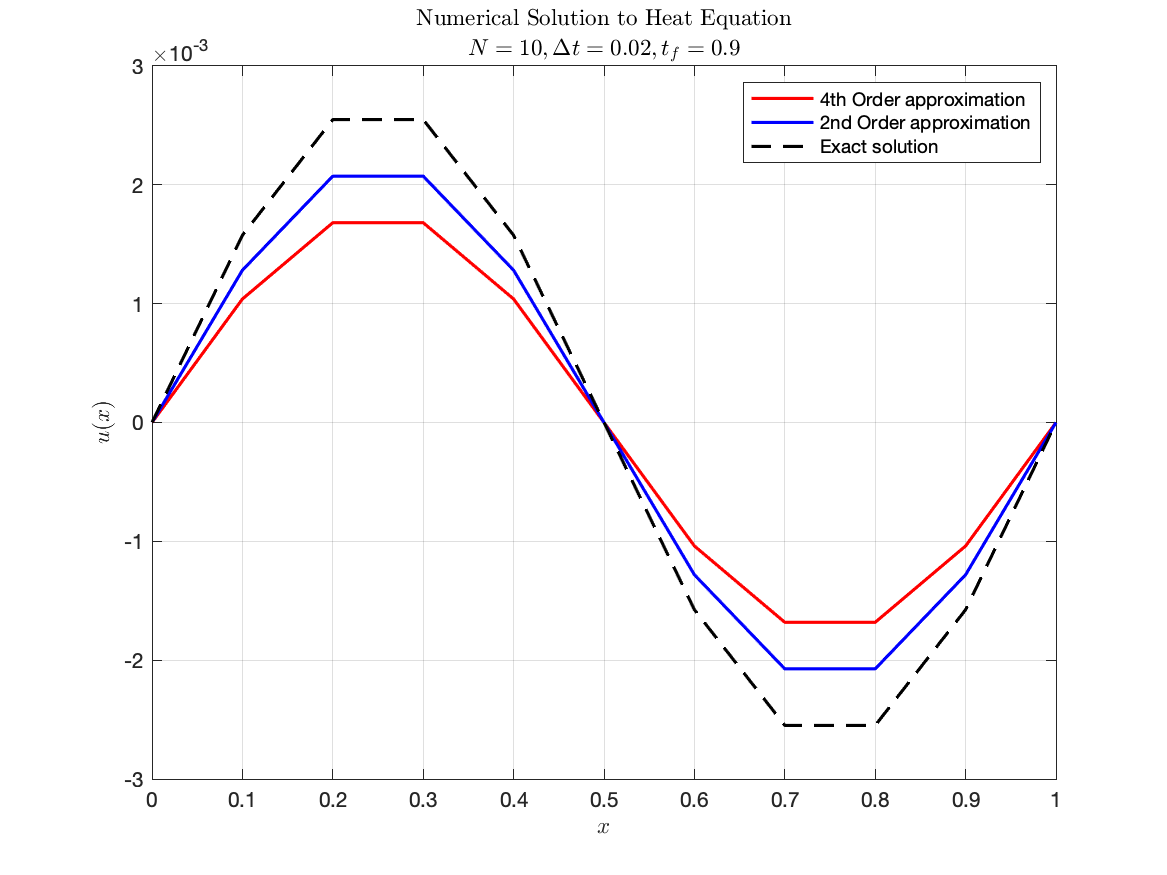
\includegraphics[width=3.8in]{q3_3}  
      \caption{Fourth Order Solution}
      \label{fig:q3b}
      \end{center}
      \end{figure}
    \item {\color{blue}Again set }$\nu=1/6$, $\dt=0.02${\color{blue}, and} $N=10$. {\color{blue}Now define ghost values using }
      \begin{align*}
        v_{-1}^n & = 0\\
        v_{N+1}^n & = 0,
      \end{align*}
      {\color{blue}and compute approximate solutions at} $t=0.06$, $t=0.1$, {\color{blue}and }$t=0.9$. \\
      
      If the ghost nodes are assigned the values of 0 each, boundary conditions are not satisfied with this approach. It can be seen in Fig~\ref{fig:q3c}. 
      
      \begin{figure}[htp]
      \begin{center}
      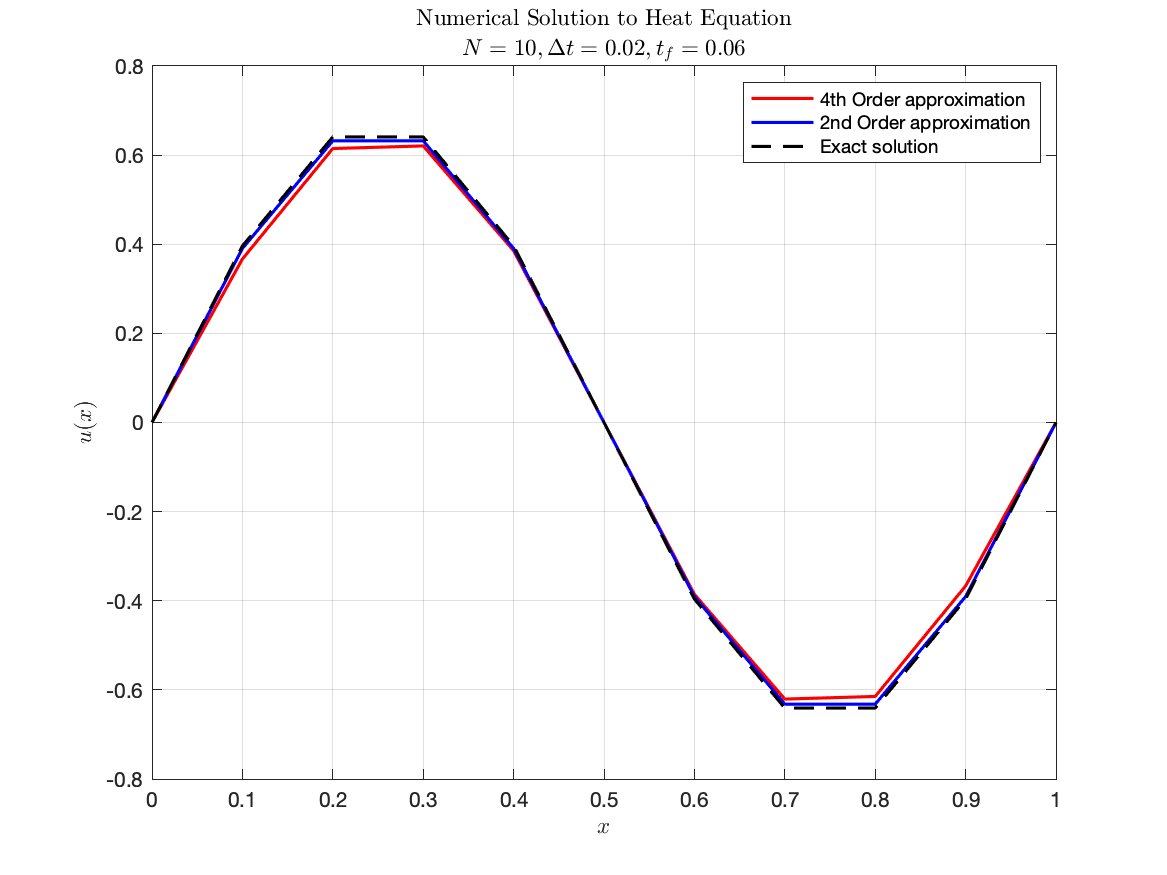
\includegraphics[width=3.8in]{q3c_1} \\
      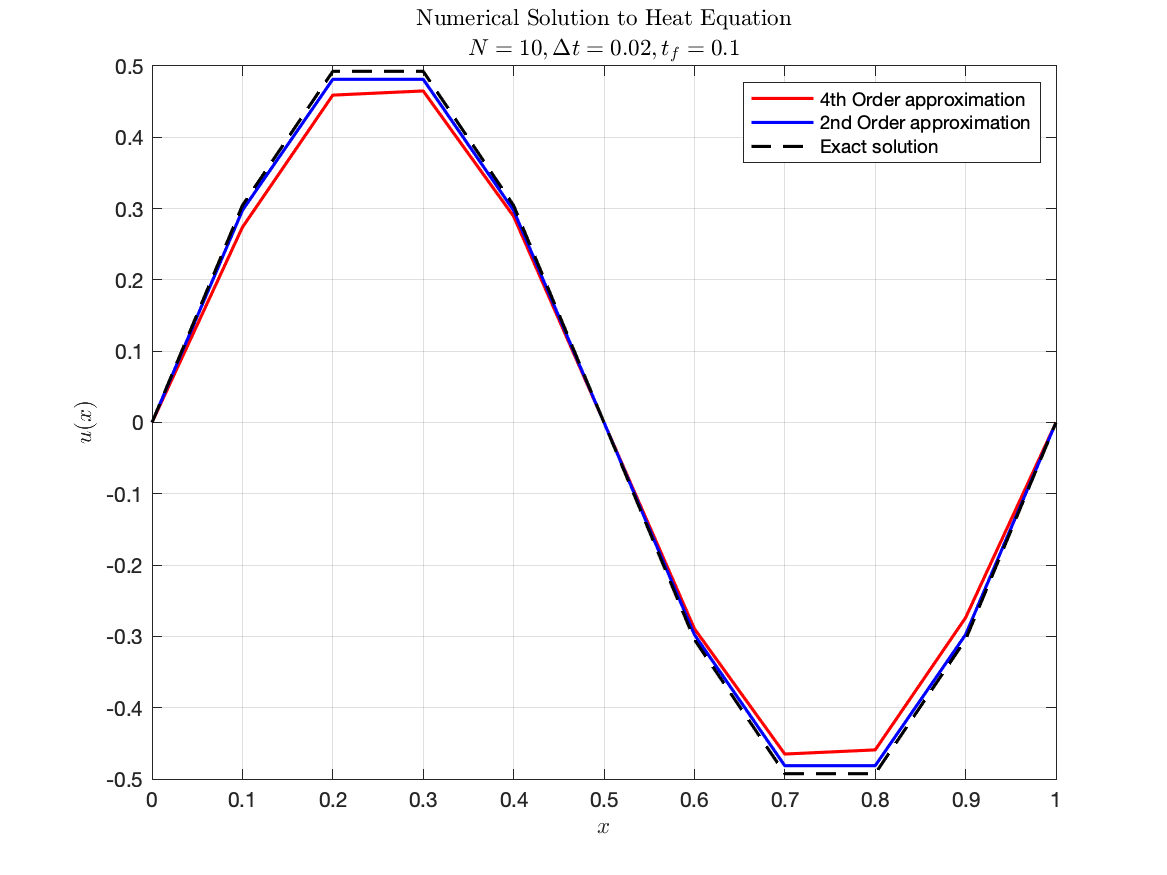
\includegraphics[width=3.8in]{q3c_2} \\
      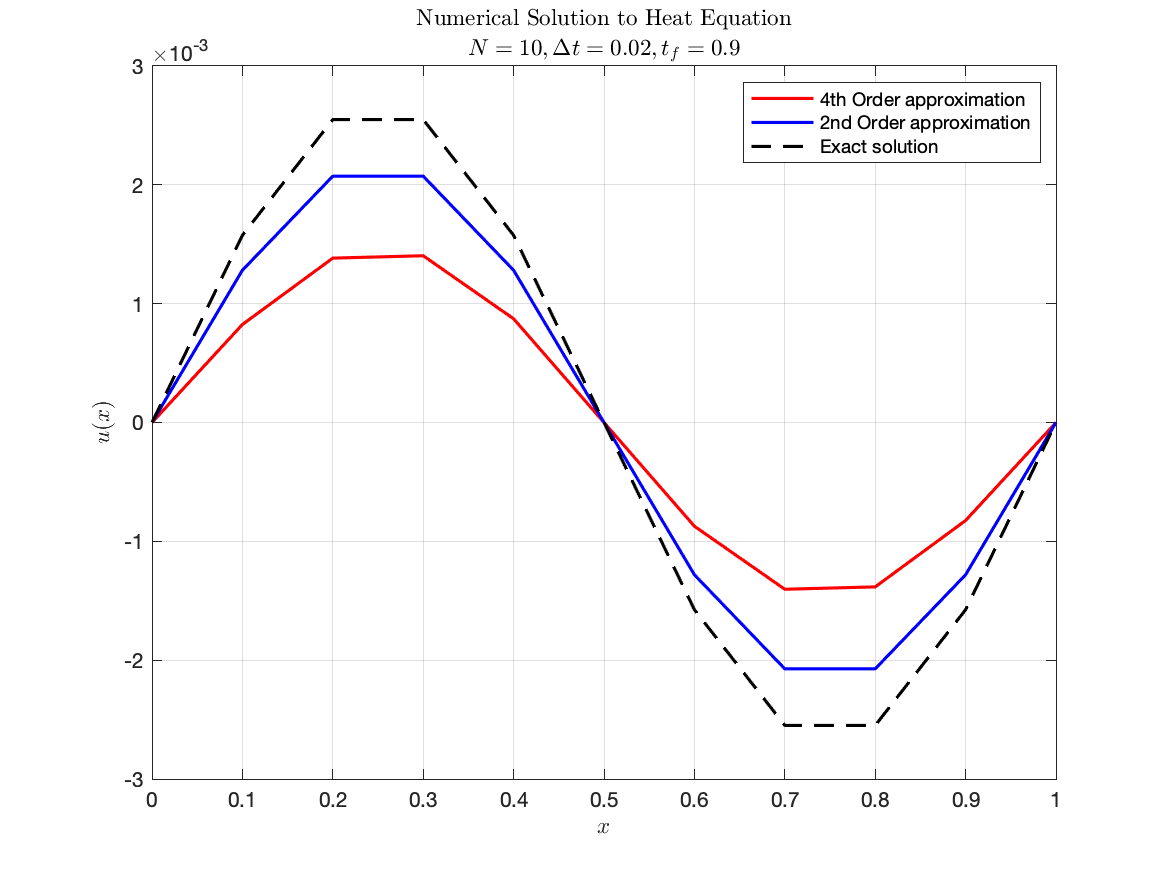
\includegraphics[width=3.8in]{q3c_3}  
      \caption{Solution with 0 values at ghost points}
      \label{fig:q3c}
      \end{center}
      \end{figure}
      
    \item {\color{blue}Discuss your results in comparison to each other and to those from PS2 \#1.} \\
    From Fig~\ref{fig:q3b}., and Fig~\ref{fig:q3c}., it does seem like the second order solution works better in terms of approximating or arriving at a numerical solution. One reason I can think of is that, by using only 2 ghost nodes and also developing a second order scheme to find the values at the ghost nodes, the overall fourth order accuracy is not met, especially at the boundaries. Maybe, adding 2 ghost nodes on either sides of the boundaries and using the developed fourth order scheme to generate the values at the boundaries might help in inching towards overall fourth order accuracy. This is my takeaway. But, it could also be that something was wrong in the way I coded this problem. But I have checked it multiple times already and I don't know if I'm missing an error that's obvious. \\
    Now, if the two fourth order schemes are compared, the scheme in which the ghost nodes are calculated using a second order accurate compatibility boundary condition (3.b), works better than the scheme where the ghost nodes are given a constant 0 value at all times. This increases my confidence in my initial guess that, if a higher order accuracy is maintained at the boundaries, the overall performance of the fourth order scheme should be better than the second order scheme. 
  \end{enumerate}
  
  %%%%%
  %%%%%
  %%%%%
  \item(15 pts.) {\color{red}Consider the heat equation}
  \[
    u_t-u_{xx}=f(x,t), \qquad 0 < x < 1, \qquad t >0
  \]
  {\color{red}with initial conditions }$u(x,t=0)=u_0(x)$ {\color{red}and boundary conditions of the form}
  \begin{align*}
    u(x=0,t) & = \gamma_L(t)\\
    u_x(x=1,t) & = \gamma_R(t).
  \end{align*}
    
  \begin{enumerate}
  
    \item {\color{blue}Determine }$f(x,t)$, $u_0(x)$, $\gamma_L(t)${\color{blue}, and} $\gamma_R(t)$ {\color{blue}so that the exact solution to the problem is }$u(x,t)=2\cos(x)\cos(t)$. \\
    
    This technique can be used to verify that the numerical solution is indeed trying to approach closer and closer to the exact analytical solution and all the tricks of adding higher order of accuracy, etc is not just to blindly ensure stability and convergence. This technique does prove that the Finite Difference approach tries to converge to the analytical/exact solution.
    
    \begin{align*}
    u(x,y) = & \ 2\cos(x)\cos(t) \\
    u(x,t=0) = & \ 2\cos(x) = u_0(x) \\
    u(x=0,t) = & \ 2\cos(t) = \gamma_L(t) \\
    u_x(x,t) = & \ -2\sin(x)\cos(t) \\
    u_x(x=1,t) = & \ -2\sin(1)\cos(t) = \gamma_R(t) 
    \end{align*}
    
    Now, 
    \begin{align*}
    u_{xx} = & \ -2\cos(x)\cos(t) \\
    u_t = & \ -2\cos(x)\sin(t) \\
    \text{Substituting it into the PDE, } \\
    u_t - u_{xx} = & \ 2\cos(x)\left(\cos(t) - \sin(t)\right) = f(x,t)
    \end{align*}
    
    \item {\color{blue}Write a code to solve this problem using the scheme}
      \[
        \Dpt v_j^n = \nu\Dpx\Dmx v_j^n+f_j^n
      \]
      {\color{blue}on the grid defined by} $x_j=j\dx$, $j=0,1,\ldots,N$, $\dx=1/N$, {\color{blue}with the parameter }$r=\Delta t/\Delta x^2$. {\color{blue}You can include ghost points as you need them, but you must ensure that your boundary conditions are at least second-order accurate.} \\
      
      To maintain second order accuracy at all nodes, two ghost nodes are added at each of the boundaries. Compatibility boundary condition at the left boundary and the central difference first derivative approximate $\Dzx$ at the right boundary will ensure second order accuracy at all node points. The code has been attached in the listing below. The scheme is developed as shown,
      \begin{align*}
      \vnpj = & \ \vnj + \frac{\dt}{\dx^2}\left(\vnjp -2\vnj + \vnjm \right) + \dt f_n^j
      \end{align*}
      
       \lstinputlisting[language=Matlab, numbers=left, stepnumber=1, firstline=1,caption={Heat Equation -Forced (Q.4)},label=code:myCode,frame=single]{HeatEqn_Forcing.m} 
       The solution at $N = 640, CFL = 0.4$, is shown in Fig~\ref{fig:q4b}. 
       \begin{figure}[htp]
	\begin{center}
      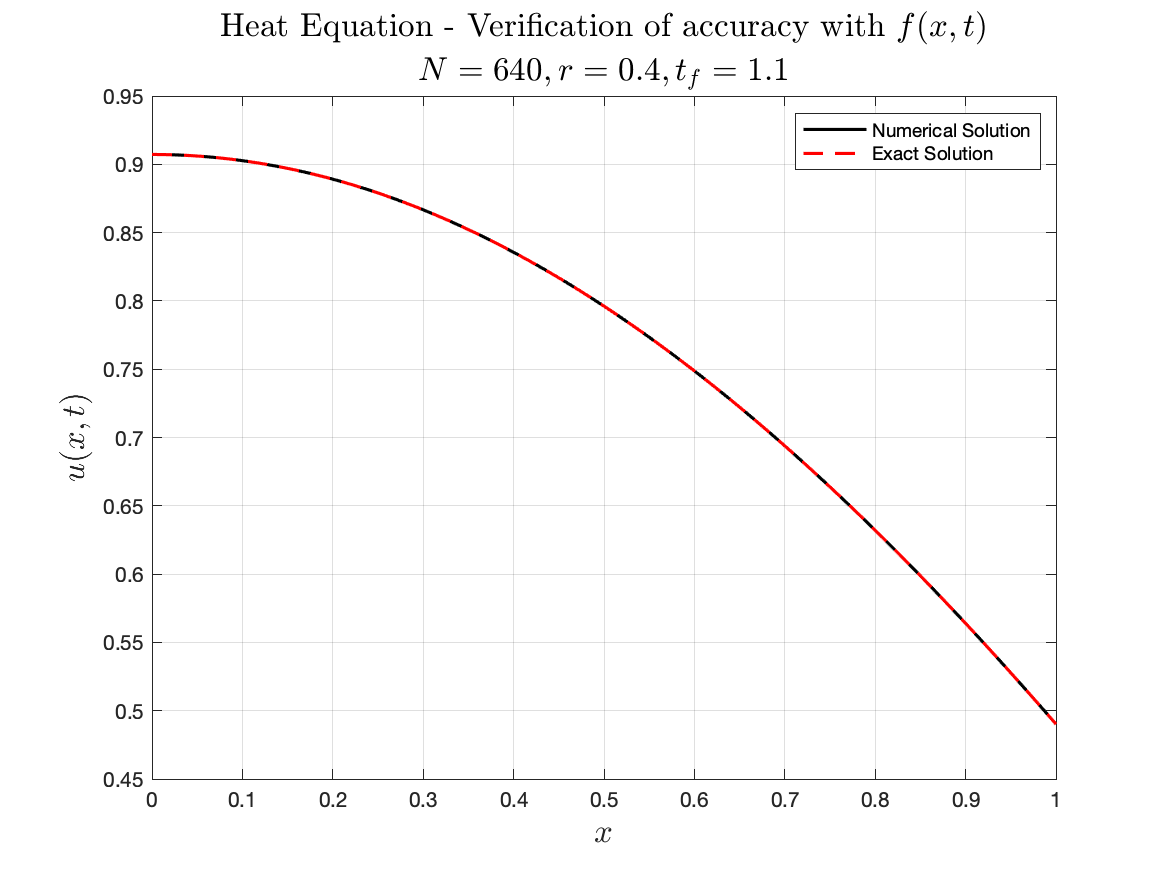
\includegraphics[width=4in]{q4_6}
      \end{center}
      \caption{Heat Equation under forcing}
      \label{fig:q4b}
       \end{figure}
      The error between the numerical solution and the exact solution is $= \ 4.9605\times10^{-5}$
      \item {\color{blue}Perform a grid refinement study using }$N=20,40,80,160, 320, 640$ {\color{blue} by computing the maximum errors in the approximation at }$t=1.1$.{\color{blue} Discuss the observed order of accuracy of the method.}\\
      
      Grid refinement study was performed and a $\log-\log$ plot is made. If the order of accuracy is $\Oc(\dx^p)$, then,
      \begin{align*}
      \text{error} = & \ k\dx^p \\
      \log(\text{error}) = & \ p\log(\dx) + \log(k) 
      \end{align*}
     The slope of this line is $p$ and it is an indication of the order of accuracy. From Fig~\ref{fig:q4}, the observed order of accuracy is approximately $1.5$.
     
     \begin{figure}[htp]
     \begin{center}
     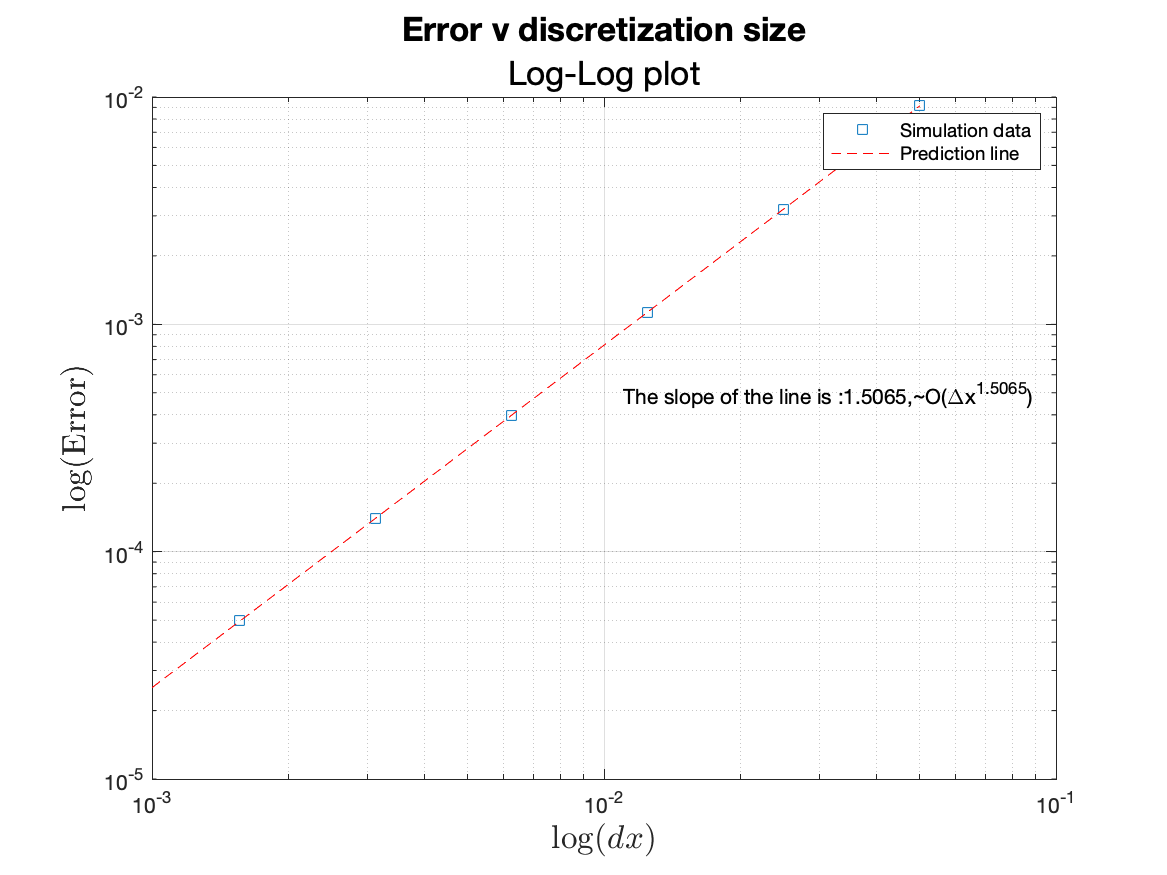
\includegraphics[width=4in]{Err_plot}
     \end{center}
     \caption{Log-Log plot of Error v spatial discretization}
     \label{fig:q4}
     \end{figure} 
      
    \end{enumerate}
\end{enumerate}


\end{document}
